\section{Saules paneļi}
% KĀ STRĀDĀ SAULES PANEĻI?
% fotons uzspīd elektronam un viņu ierosina un tad tas aiziet pāri vadītspējas zonai un aizpeld uz elektrodu un caurums aizpeld uz otru elektrodu un rodas potenciālu starpība no kurienes strāva.
% Ielikt dokus par LG un JA tipu + no kādiem kristāliem tie
% Ielikt shēmu
% analīze par saules paneļu plantācijām pasaulē
% optimālie apstākļi?

Saules paneļi sastāv no fotoelementiem, kas pārveido gaismas enerģiju elektriskā lauka enerģijā. Fotoelements, kura uzbūves shēma ir parādīta \ref{fig:PV}. attēlā, ir p-n pāreja ar elektriskajiem kontaktiem, kas pieslēgti pie lādētāja vai cita enerģijas patērētāja. Fotoelementa apakšējā daļa sastāv no n-tipa pusvadītāja, kurā lādiņa pamatnesēji ir elektroni, bet augšējā daļa -- no p-tipa pusvadītāja, kur lādiņa pamatnesēji ir caurumi. 

\begin{figure}[h]
    \centering
    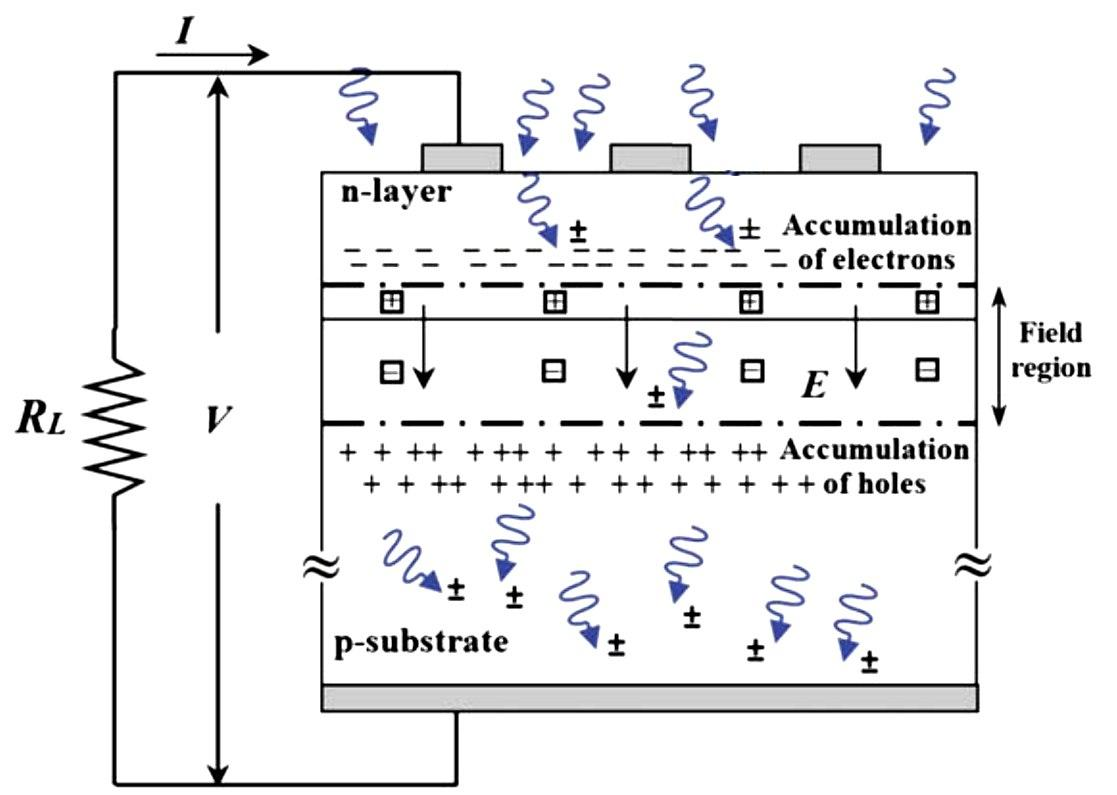
\includegraphics[width=0.6\linewidth]{figures/misc/PV.jpg}
    \caption{Saules paneļa shēma. Tas sastāv no fotoelementiem, kuru augšējais slānis veidots no p-tipa pusvadītāja, bet apakšējais --- no n-tipa pusvadītāja~\cite{Yahyaoui}.}
    \label{fig:PV}
\end{figure}

P-tipa un n-tipa pusvadītāja īpašības var panākt, piemēram, dopējot silīcija kristālu ar attiecīgi III vai V grupas elementiem. Ja silīcija kristālam pievieno bora atomus nelielā koncentrācijā, izveidojas \ref{fig:p-n-type}. att. pa kreisi redzamā situācija. Katram Si atomam ir četri elektroni ārējā čaulā, ar kuru palīdzību atoms izveido četras kovalentās saites ar četriem citiem atomiem. Savukārt bors, būdams III grupas elements, var izveidot tikai trīs saites. Tādā veidā pie bora atoma parādās "caurums" -- nenoslēgta kovalentā saite, kas attēlā apzīmēta ar sarkanu apli. Uz šo vietu var pārvietoties kāds no blakus esošiem elektroniem, bet tad neaizpildīta vieta parādīsies pie blakus esošā atoma. Tādā veidā var uzskatīt, ka caurums pārvietojas, un nosaukt to par pozitīvo lādiņa nesēju. Šādus pusvadītājus sauc par p-tipa pusvadītājiem. ~\cite{Yahyaoui}

Ja silīcija kristālam pievieno fosfora atomus, izveidojas pretēja situācija -- pie P atoma parādās elektrons, kas nepiedalās saites veidošanā (sk. att. \ref{fig:p-n-type}., pa labi). Lai pārvietotos, brīvajam elektronam ir nepieciešams mazāk enerģijas nekā elektroniem, kas veido kovalentās saites starp Si atomiem. Tātad, lādiņa pamatnesēji n-tipa pusvadītājos ir elektroni.

Dopējot divus blakus esošus Si kristāla apgabalus dažādā veidā, iegūst p-n pāreju. Uz robežas starp apgabaliem elektroni no n-tipa apgabala var rekombinēties jeb difūzijas ceļā nokļūt uz p-tipa apgabalu un aizpildīt pietiekami tuvu esošus caurumus, tāpēc p-tipa pusvadītājā mala uzlādējas negatīvi.

\begin{figure}[h]
	\centering
	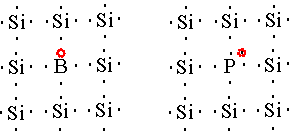
\includegraphics[width=0.5\linewidth]{figures/misc/p_n_type.pdf}
	\caption{Silīcija kristāla 2D izklājums, atomu ārējās čaulas elektroni ir apzīmēti ar punktiem. Pievienojot bora atomu, iegūst p-tipa pusvadītāju (pa kreisi), bet fosfora atomu --- n-tipa pusvadītāju (pa labi).}
	\label{fig:p-n-type}
\end{figure}

Fotoelementa darbība balstās uz iekšējo fotoelektrisko efektu -- parādību, kad elektrons tiek ierosināts ar gaismas kvantu un pāriet no valences zonas uz vadītspējas zonu. Kad tas notiek augšējā slānī (p-tipa pusvadītājā), elektrons atgrūžas no robežas starp slāņiem, kura ir negatīvi lādēta rekombinācijas dēļ. Negatīvi lādētā (no p-tipa pusvadītāja puses) robeža rada potenciālu starpību, kas veicina elektronu kustību pa vadiem uz patērētāju, tādā veidā radot elektrisko strāvu.

\subsection{Paneļu veidi}

Darbā ir apskatīti divi Saules paneļu veidi. Ražotāju referenču lapās LG tiek prognozēta labāka atdeve saulainās dienās~\cite{LGtips}, bet JA labāka atdeve vājas gaismas intensitātes vidēs~\cite{JAtips}.

\begin{table}[h]
    \caption{JA un LG paneļu tipu salīdzinājums~\cite{JAtips}~\cite{LGtips}} % uzrakstīt kādu absolūto TSI izmērīja vai norādīt uz grafiku?
    \begin{center}
    \begin{tabular}{| r | c | c |}
    \hline
    Tips & JA & LG \\ \hline
    Modelis &  JAP60-275/4BB & LG365Q1C-A5\\ \hline
    % materiāls & silikons &   \\ \hline
	Kristāla veids & Polikristālisks & Monokristālisks \\ \hline
	% šūnas izmērs, mm  &156x156  & \\ \hline
	Šūnu skaits  &60  &60 \\ \hline
	Virsmas laukums, $m^2$ &1.64  &1.72 \\ \hline
	STC Pmax, $W$ 	&270 &365\\ \hline
	NOCT Pmax, $W$  &196 &275\\ \hline
	Efektivitāte, \% &16 & 20\\ \hline
    \end{tabular}
    \end{center}
    \label{tab:ja_lg_tipi}
\end{table}

Paneļu maksimālā jauda ($P_{max}$) tiek testēta pie:
\begin{itemize}
\item standarta testa nosacījumiem (\textit{Standart test condition} - STC):\\
Saules izstarojums 1000 W/m$^2$; apkārtējā temperatūra 25\textdegree C.
\item nominālās šūnas darba temperatūras (\textit{Nominal operating cell temperature} - NOCT):\\
Saules izstarojums 800 W/m$^2$; apkārtējā temperatūra 20 \textdegree C; vēja ātrums 1 m/s
\end{itemize}

% ielikt bildi ar to kas saules apstarojumā pazūd no imene

% \begin{figure}[h]
%     \centering
%     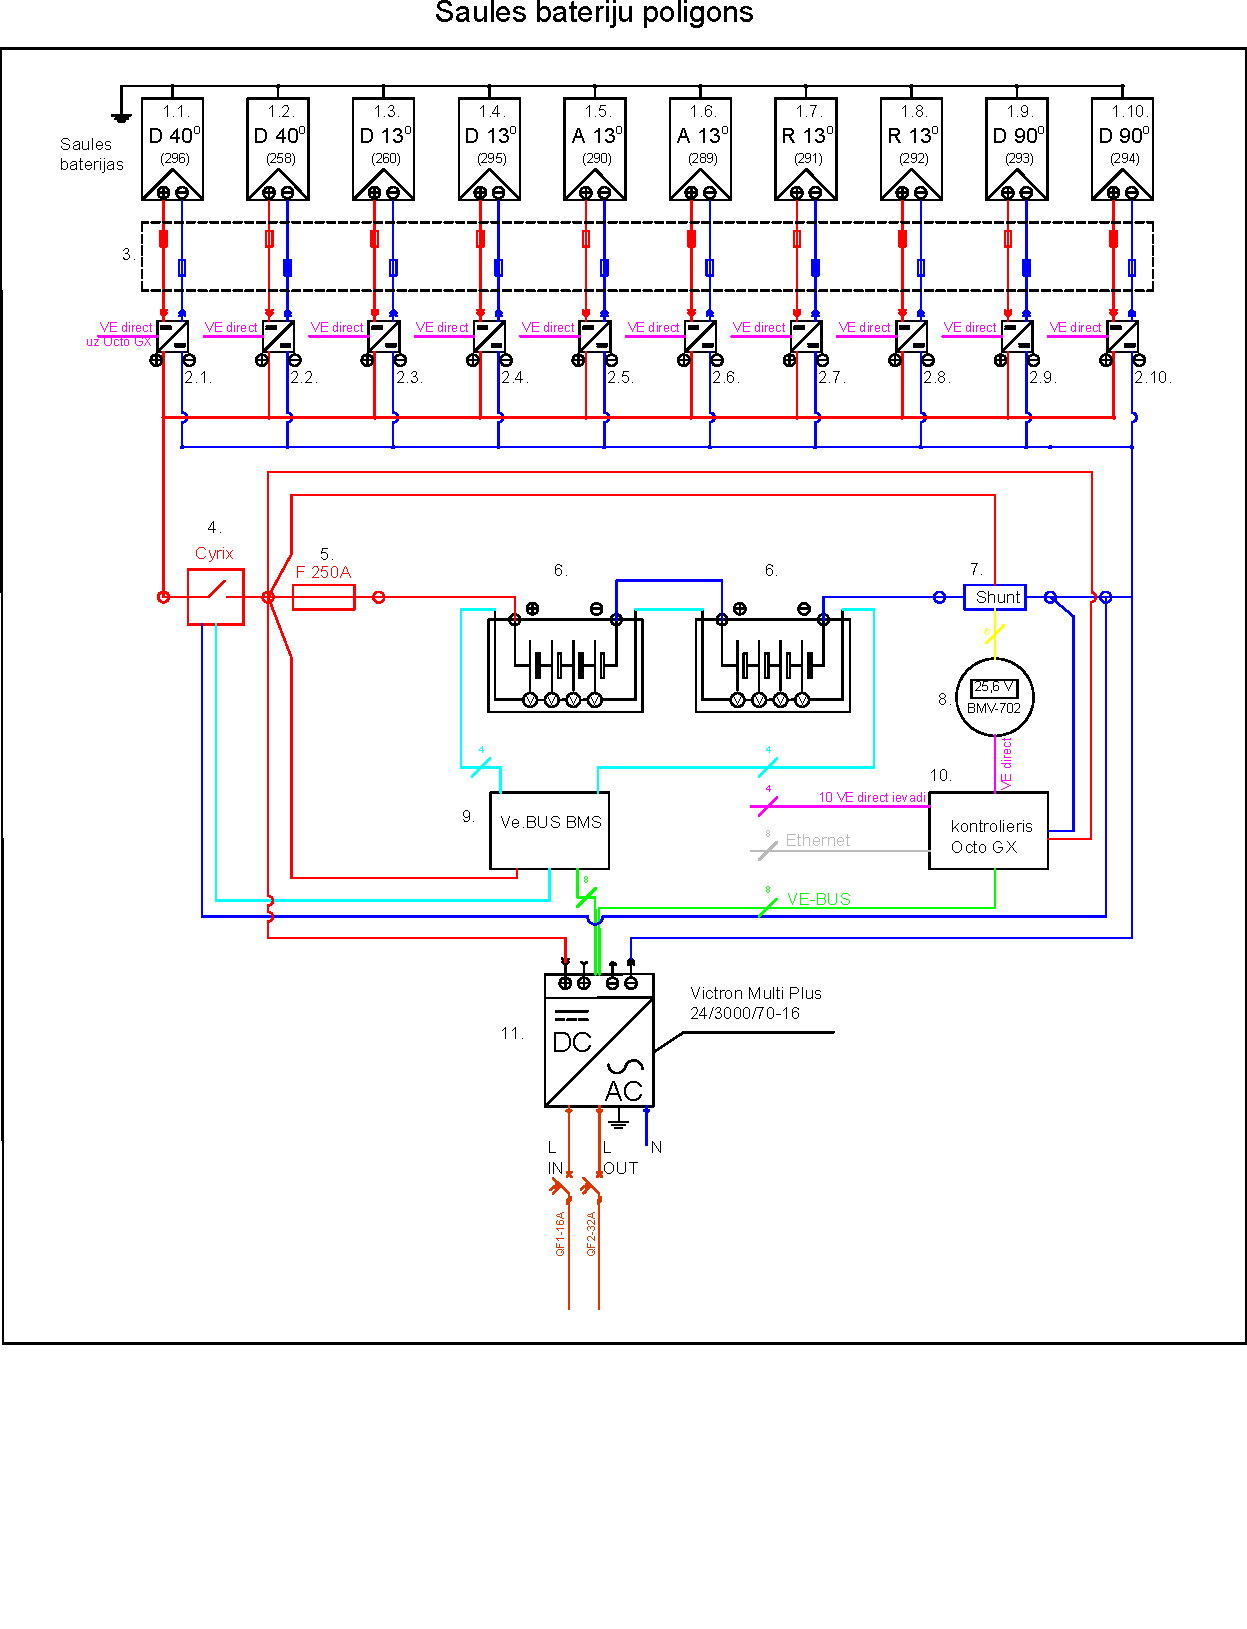
\includegraphics[width=0.7\linewidth]{figures/misc/shema.pdf}
%     \caption{Saules paneļu elektriskā shēma}
%     \label{fig:paneli666}
% \end{figure}

\begin{figure}[h]
    \centering
    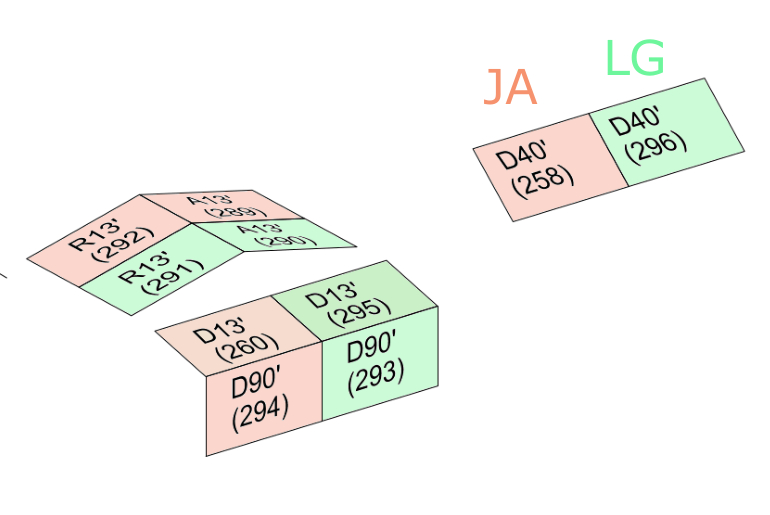
\includegraphics[width=0.7\linewidth]{figures/misc/uzstadijumaShema.jpg}
    \caption{Saules paneļu telpisko orientāciju shēma}
    \label{fig:paneli}
\end{figure}

\begin{figure}[h]
    \centering
    \includegraphics[width=0.7\linewidth]{figures/stenduBildes/overview2.JPG}
    \caption{Saules paneļu telpiskās orientācijas dabā (autors Māris Šinka)}
    \label{fig:paneli}
\end{figure}

\subsection{Saules paneļu izmantošana pasaulē}

Silīcija Saules paneļu attīstības intensīvākais posms bija apmēram no 1980. līdz 2000. gadam, kad to maksimālā efektivitāte palielinājās no 15\% līdz 25\%
\cite{Sivaram}. Nākamajos 20 gados efektivitātes pieaugums bija gandrīz desmit reizes mazāks. Tiek pētīti arī citi Saules paneļu pusvadītāju veidi, piemēram CdTe vai GaAs, tomēr monokristāliskā un polikristāliskā silīcija Saules paneļi joprojām aizņem lielāko daļu no tirgus, piemēram, Vācijā Si sastādīja vairāk nekā 90\% no Saules paneļu tirgus pēdējo septiņu gadu laikā ~\cite{prognoze}. Tas tādēļ, ka Si ir pieejamāks un lētāks nekā GaAs\cite{hayes_clemens_2015}, un vairāk izpētīts nekā CdTe pusvadītāji~\cite{Sivaram}.

Svarīgi ievērot, ka Saules paneļu efektivitāte ir atkarīga no vairākiem faktoriem, kas mainās līdz ar ģeogrāfisko novietojumu: ģeogrāfiskā platuma, gadalaika, mākoņainības un gaisa piesārņojuma. Tātad, detalizēta Saules paneļu efektivitātes analīze var būt noderīga katrā valstī, lai precīzāk izvērtētu solārās enerģijas lietošanas perspektīvas tajā. Var minēt dažus šādu pētījumu piemērus.
\begin{itemize}
  \item Indijas pilsētā Bangalorē izpētīja, ka efektivitāte musona un pēc-musona periodos ir augstāka, nekā ziemā un vasarā. To var saistīt ar lielu nokrišņu daudzumu musona periodā, kas labi dzesē Saules paneļus, un ar lielāku saulaino dienu skaitu pēc-musona periodā~\cite{effectCloudsOnSurface}.
  \item Eksperiments Mumbajā \cite{improvePerformance} ļauj secināt, ka karsts un sauss klimats ne tikai samazina enerģijas pārvērtības lietderības koeficientu, bet arī izraisa defektus un silīcija bojājumus, kas palielina enerģijas zudumus. Tiek norādīts, ka šādā klimatā tipiskais Saules paneļu dzesēšanas risinājums -- ūdens izsmidzināšana -- nav pielietojams, jo tieši šādā klimatā ūdens trūkums ir svarīga problēma.
  \item Indonēzijā pētnieki novēroja, ka mitruma un vēja ātruma palielināšana samazina Saules paneļu efektivitāti~\cite{improvePerformance}.
  \cite{Sani_2018}. Atšķirībā no iepriekšējā pētījumā, aplūkotajā temperatūras apgabalā (42 -- 52 \textdegree C) temperatūra pozitīvi korelē ar paneļu efektivitāti, kas iespējams saistīts ar GHI palielināšanos. 
  \item Arī Latvijā jau ir uzstādītas saules paneļu sistēmas. Piemēram, Ulbrokā 2017. gadā 20 paneļu sistēma kopā saražoja 4554.06 kWh -- vidēji 227.703 kWh gadā no viena paneļa (skat.~\ref{fig:ulbroka}).
\end{itemize}


\begin{figure}[h]
  \centering
  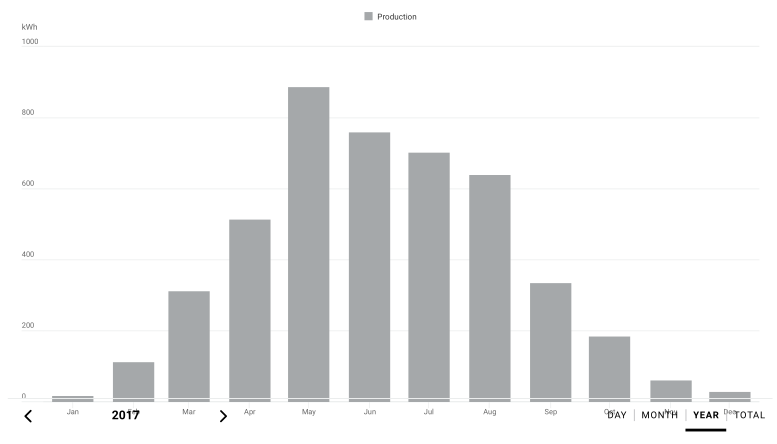
\includegraphics[width=\linewidth]{figures/misc/2017.png}
  \caption{20 Saules paneļu sistēmas saražotā enerģija Ulbrokā 2017. gadā. Virziens: D, leņķis 15 grādi \cite{fronius}}
  \label{fig:ulbroka}
\end{figure}

\section{Darba aktualitāte}

Latvijā veikto pētījumu daudzums un kvalitāte pagaidām neļauj iegūt pilnīgu priekšstatu par Saules paneļu lietošanas iespējām un prognozēt dažādu paneļu tipu efektivitāti reālā Latvijas klimatā. Tāpēc šī darba novitāte ietverta programmatūras izveidē, kas ļauj attēlot un apstrādāt Saules paneļu monitoringa datus, kas dos iespēju veikt turpmākus dziļākus pētījumus par dažādiem solārās enerģijas pielietojuma aspektiem Latvijā.

